\scanpage{69}\mspage{68}
% Figure F01: the opening paragraph, with both insertion arms and the small
% detached stroke below stonienne. Words occur once in this group.
\figure{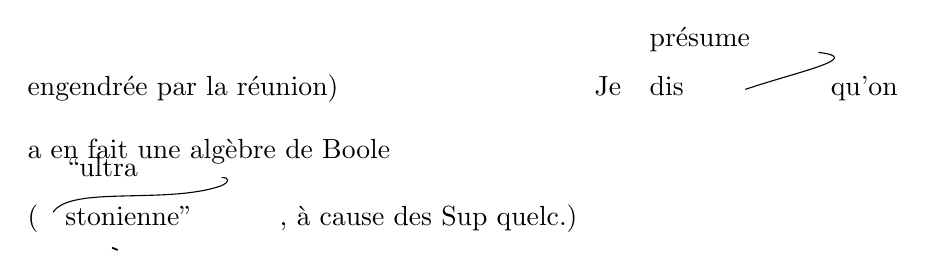
\begin{tikzpicture}[x=1cm,y=1cm,every node/.style={anchor=base west,inner sep=0pt}]
\node at (0,0) {engendrée par la réunion)};
\node at (7.2,0) {Je};
\node at (7.9,0) {\deleted{dis}};
\node at (7.9,0.62) {\inserted{présume}};
\node at (10.2,0) {qu'on};
\draw (10.05,0.55) .. controls (10.65,0.48) and (9.8,0.31) .. (9.12,0.08);
\node at (0,-0.8) {a en fait une algèbre de Boole};
\node at (0,-1.65) {(};
\node at (0.48,-1.65) {stonienne''};
\node at (0.48,-1.02) {\inserted{``ultra}};
\draw (0.33,-1.48) .. controls (0.55,-1.14) and (1.75,-1.38) .. (2.45,-1.15)
 .. controls (2.58,-1.10) and (2.57,-1.03) .. (2.47,-1.04);
\draw[line width=0.65pt] (1.08,-1.93)--(1.15,-1.96);
\node at (3.2,-1.65) {, à cause des $\mathrm{Sup}$ quelc.)};
\end{tikzpicture}}

% slanted left margin note
\margin{Cela sera valable dans ``le cas ensembliste'', et en tous cas dans les exemples types, donnés \deleted{\unsure{tout}} au début, en termes d'un $E$ (top. ou mesurable), alors $\Sigma$ s'identifie à l'ens des parties de $E$, et \unsure{on trouve|on trouvera|on retrouve} le compactifié de \unsure{Stone} de $E_{\mathrm{disc.}}$ Dans le cas qui vient, \unsure{je} ne vois comment \unsure{prouver}, pour trois supports
\[
P,Q,R\quad P\wedge(Q\vee R)=\unsure{\{|(}(P\wedge Q)\vee(P\wedge R)\unsure{\}|.|,|)}
\]}

\deleted{Il faudra y revenir}

\unsure{Donc} les supports s'identifient aux \unsure{Parties|Partie} à la fois ouvertes et fermées du spectre, qui serait un espace \deleted{\unsure{to|tot}}\unsure{cpct|cpt|compact} \deleted{\unsure{tot}} \unsure{disconnexe} ultra.stonien.

L'involution correspond au passage au complémentaire.

On fera attention que la construction $\Sigma$ ne dépend que de l'ens ordonné
% Figure F02: the complete compatibility insertion, its enclosure, and the
% lower toute insertion and angular leader. Adjoining words occur once.
\figure{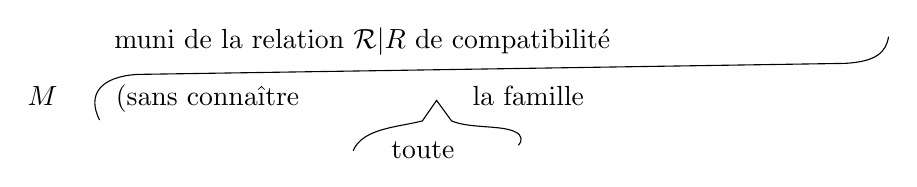
\begin{tikzpicture}[x=1cm,y=1cm,every node/.style={anchor=base west,inner sep=0pt}]
\node at (0,0) {$M$};
\node at (1.12,0) {(sans connaître};
\node at (5.65,0) {la famille};
\node at (1.10,0.72) {\inserted{muni de la relation $\unsure{\mathcal R|R}$ de compatibilité}};
\draw (0.92,-0.19) .. controls (0.76,0.13) and (0.92,0.36) .. (1.40,0.39)
 -- (10.38,0.53) .. controls (10.78,0.55) and (10.91,0.67) .. (10.94,0.87);
\node at (4.62,-0.68) {\inserted{toute}};
\draw (4.14,-0.58) .. controls (4.26,-0.29) and (4.72,-0.28) .. (5.02,-0.20)
 -- (5.20,0.06) -- (5.39,-0.20)
 .. controls (5.62,-0.30) and (6.02,-0.25) .. (6.20,-0.34)
 .. controls (6.29,-0.38) and (6.29,-0.46) .. (6.24,-0.51);
\end{tikzpicture}}
des parties $\unsure{\Phi'|\overline\Phi|\Phi}$ de $M$, correspondant aux figures). En effet, en termes de $(M,\leq,R)$, le cosupport d'une partie $M'$ de $M$ est défini par
\[
\operatorname{cosup}_M(M')=\{\,x\in M\mid(x,x')\in\mathcal R\quad\forall x'\in\unsure{M'|M''}\,\}
\]

% Figure F03: slanted bottom margin note and its separate, nearly horizontal
% rule in the page's orientation. The words are not duplicated in a margin macro.
\figure{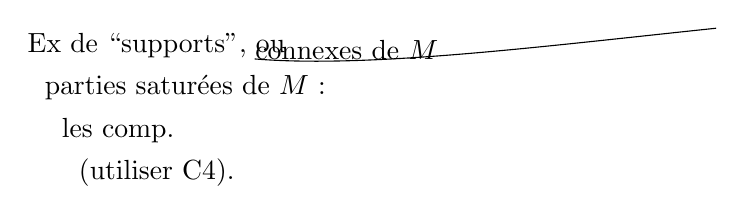
\begin{tikzpicture}[x=1cm,y=1cm,every node/.style={anchor=base west,inner sep=0pt}]
\begin{scope}[rotate=22]
\node at (0,0) {\uline{Ex} de ``supports'', ou};
\node at (0,-0.58) {parties saturées de $M$ :};
\node at (0,-1.16) {les comp.};
\node at (2.65,-1.16) {connexes de $M$};
\node at (0,-1.74) {(utiliser C4).};
\end{scope}
\draw (2.89,-0.08) .. controls (4.35,-0.20) and (6.55,0.08) .. (8.75,0.31);
\end{tikzpicture}}
